\documentclass[11pt,a4paper]{article}

\usepackage[margin=2.2cm]{geometry}
\usepackage[T1]{fontenc}
\usepackage{lmodern}
\usepackage{microtype}
\usepackage{amsmath,amssymb}
\usepackage{booktabs}
\usepackage{tabularx}
\usepackage{multirow}
\usepackage{enumitem}
\usepackage{caption}
\usepackage{placeins}
\usepackage[table]{xcolor}
\usepackage{tikz}
\usetikzlibrary{arrows.meta,positioning,calc,fit,backgrounds,shapes.geometric,decorations.pathreplacing}
\usepackage{pgfplots}
\pgfplotsset{compat=1.16}
\usepackage[hidelinks]{hyperref}

\setlist{itemsep=2pt,topsep=4pt}
\makeatletter
\setlength\@fptop{0pt}\setlength\@fpsep{14pt plus 2pt}\setlength\@fpbot{0pt plus 1fil}
\makeatother
\newcommand{\code}[1]{\texttt{#1}}
\newcommand{\vect}[1]{\mathbf{#1}}
\newcolumntype{L}{>{\raggedright\arraybackslash}X}
\newcolumntype{C}{>{\centering\arraybackslash}p{6.2mm}}
\tikzset{
  box/.style={draw, rounded corners=2pt, align=center, font=\small, minimum height=8mm, inner sep=3pt, fill=white},
  data/.style={box, fill=gray!12},
  model/.style={box, fill=blue!8},
  stp/.style={box, fill=orange!10},
  arr/.style={-{Stealth[length=2mm]}, thick},
  note/.style={font=\footnotesize\itshape, align=center, text=black!70}}
% per-query outcome cells
\newcommand{\Y}{\cellcolor{green!25}\textbf{H}}
\newcommand{\N}{\cellcolor{red!12}n}
\newcommand{\W}{\cellcolor{red!25}w}
\newcommand{\B}{\cellcolor{yellow!35}b}

\title{Semantic Embedding on a Frozen Gaussian Splat:\\[2pt]
\large The Complete Pipeline and a Comparison of Four Teacher Designs (Old, A, B2, C2)}
\author{Suhan --- Team Radiance, Department of Computer Science and Engineering,\\University of Moratuwa}
\date{8 October 2026}

\begin{document}
\maketitle

\begin{abstract}
Our drone-simulation pipeline (FiGS / SOUS-VIDE) turns a phone capture of a room into a 3D Gaussian Splat. The
semantic layer described here attaches language-aligned features to that splat --- without changing it --- so that an
operator can type a phrase such as ``red cup'' and obtain a 3D goal and a safe approach waypoint. This report documents
the whole process end to end: inputs and camera refinement, the 2D teacher features (CLIP, DINOv2 and, in one design,
SAM), the two ways of attaching them to Gaussians (the training-free \emph{lift} and the trained \emph{FMGS} field),
the stored table, the query, the evaluation protocol and every measurement. Four designs of the CLIP teacher are
compared on two scenes and four backends: \textbf{Old} (a scale-averaged crop pyramid), \textbf{A} (crop scales kept in
three groups, the group chosen per query), \textbf{B2} (CLIP on SAM segments, by size level, with the pyramid filling
uncovered cells) and \textbf{C2} (a larger CLIP, ViT-L/14, with a calibrated relevancy floor). At the default query
settings the lift finds 20, 22, 21 and 19 of 29 annotated objects respectively, and FMGS 8--15. A floor sweep shows that
most of the differences between teachers are differences in how their relevancy relates to the fixed 0.55 floor: at an
equal number of false detections the four designs are within two objects of each other, with B2 (without level choice)
reaching 24 of 29. FMGS misses mainly because its high-relevancy Gaussians are scattered over the room. We explain each
observation and propose improvements for each pipeline and for combinations.
\end{abstract}

\noindent\textbf{Companion document.} \code{semantics\_primer.pdf} explains Gaussian splats, CLIP, DINOv2, SAM, the lift
and FMGS at an abstract level; this report assumes it.

\tableofcontents
\newpage

%=======================================================================================
\section{Goal, constraints and terminology}
%=======================================================================================

The project's aim is \emph{language-guided goals for simulation-trained visuomotor drone policies}. A course (a list of
keyframes) is flown by an expert controller in the splat's photo-realistic renders; those flights train the SV-Net
student policy. The semantic layer lets an operator \emph{name} a target instead of placing it by hand: the system
finds the object in 3D and appends an approach point to the course.

\paragraph{Constraints that shaped every decision.}
\begin{enumerate}
  \item \textbf{The splat is frozen.} Courses, cached renders and trained policies depend on its exact Gaussians;
        semantics are attached on top and never by retraining it. The FMGS trainer checksums the Gaussians before and
        after training to prove it.
  \item \textbf{Open vocabulary.} No object list and no labels: any phrase CLIP understands is a valid query.
        Annotations are used only to \emph{score}.
  \item \textbf{One 8\,GB GPU} (RTX~2080, sm\_75) for building, on a shared machine with one GPU job at a time; queries
        run in a CPU-only worker so they never compete with simulation.
  \item \textbf{A pinned software stack} (torch~2.1.2 / CUDA~11.8, nerfstudio~1.1.4, gsplat~1.0.0, tiny-cuda-nn~2.0,
        open\_clip~2.24.0). Two of its limits recur below: gsplat's backward pass handles at most 32 feature channels,
        and tiny-cuda-nn on sm\_75 cannot launch a 192-dimensional hash grid.
\end{enumerate}

\paragraph{Names used throughout.}
\begin{itemize}
  \item \textbf{Teachers}: the CLIP design. \emph{Old}, \emph{A}, \emph{B}, \emph{B2}, \emph{C}, \emph{C2}
        (Section~\ref{sec:teachers}). The report focuses on Old, A, B2 and C2; B and C are the first versions of B2 and C2
        and are included where they explain a change.
  \item \textbf{Backends / variants}: \textbf{L-C} lift, CLIP-only query; \textbf{L-CD} lift with DINOv2 used at query
        time; \textbf{F-C} FMGS trained on CLIP alone; \textbf{F-CD} FMGS with its paper losses (CLIP + DINO + pixel
        alignment). A suffix \emph{flat} means the same table queried without per-query scale or level choice.
\end{itemize}

%=======================================================================================
\section{The pipeline end to end}
%=======================================================================================

\begin{figure}[ht]
\centering
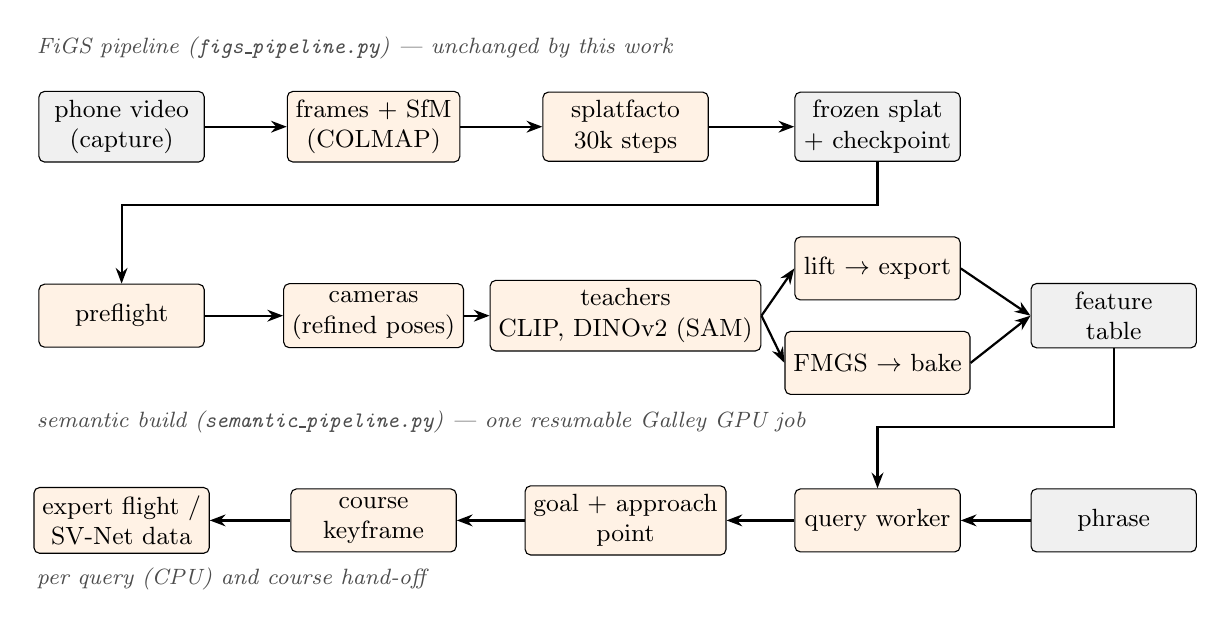
\begin{tikzpicture}[font=\small, every node/.append style={minimum width=2.1cm}]
  % row 1: FiGS
  \node[note, anchor=west] at (-1.2,1.0) {FiGS pipeline (\code{figs\_pipeline.py}) --- unchanged by this work};
  \node[data] (cap) at (0,0) {phone video\\(capture)};
  \node[stp] (sfm) at (3.2,0) {frames + SfM\\(COLMAP)};
  \node[stp] (spl) at (6.4,0) {splatfacto\\30k steps};
  \node[data] (splat) at (9.6,0) {frozen splat\\+ checkpoint};
  % row 2: semantic build
  \node[note, anchor=west] at (-1.2,-3.75) {semantic build (\code{semantic\_pipeline.py}) --- one resumable Galley GPU job};
  \node[stp] (pre) at (0,-2.4) {preflight};
  \node[stp] (cams) at (3.2,-2.4) {cameras\\(refined poses)};
  \node[stp] (teach) at (6.4,-2.4) {teachers\\CLIP, DINOv2 (SAM)};
  \node[stp] (lift) at (9.6,-1.8) {lift $\rightarrow$ export};
  \node[stp] (fmgs) at (9.6,-3.0) {FMGS $\rightarrow$ bake};
  \node[data] (table) at (12.6,-2.4) {feature\\table};
  % row 3: per query
  \node[note, anchor=west] at (-1.2,-5.75) {per query (CPU) and course hand-off};
  \node[stp] (fly) at (0,-5.0) {expert flight /\\SV-Net data};
  \node[stp] (course) at (3.2,-5.0) {course\\keyframe};
  \node[stp] (goal) at (6.4,-5.0) {goal + approach\\point};
  \node[stp] (query) at (9.6,-5.0) {query worker};
  \node[data] (text) at (12.6,-5.0) {phrase};
  \draw[arr] (cap) -- (sfm); \draw[arr] (sfm) -- (spl); \draw[arr] (spl) -- (splat);
  \draw[arr] (splat.south) -- ++(0,-0.55) -| (pre.north);
  \draw[arr] (pre) -- (cams); \draw[arr] (cams) -- (teach);
  \draw[arr] (teach.east) -- (lift.west); \draw[arr] (teach.east) -- (fmgs.west);
  \draw[arr] (lift.east) -- (table.west); \draw[arr] (fmgs.east) -- (table.west);
  \draw[arr] (table.south) -- ++(0,-1.0) -| (query.north);
  \draw[arr] (text) -- (query); \draw[arr] (query) -- (goal); \draw[arr] (goal) -- (course); \draw[arr] (course) -- (fly);
\end{tikzpicture}
\caption{From a capture to a flyable semantic goal. The upper row is the existing FiGS pipeline; the middle row is the
semantic build (one resumable GPU job in Galley); the lower row runs per query on the CPU.}
\label{fig:e2e}
\end{figure}

Figure~\ref{fig:e2e} shows the whole chain. The semantic build is driven by \code{figs/semantic\_pipeline.py}, which runs
a fixed sequence of steps per scene and backend (Table~\ref{tab:steps}). Each step writes a fingerprint (its inputs and
settings); a step whose fingerprint is unchanged is skipped, so an interrupted build resumes where it stopped (this
mattered: a lightning-induced power cut interrupted one Phase~5 run). Each step runs in a child process that prints
\code{GALLEY\_JSON} progress lines which Galley parses for its job view, and VRAM is sampled device-wide.

\begin{table}[ht]
\centering\small
\begin{tabularx}{\linewidth}{@{}lLl@{}}
\toprule
Step & What it does & Output \\
\midrule
preflight & finds the scene's active run and checkpoint; computes the table key (run + checkpoint + mtime = Galley's
\code{.splat} cache key) & scene record \\
cameras & loads the checkpoint, applies splatfacto's learned pose corrections (\code{optimized\_c2w}), checks
rendered PSNR refined vs raw & refined cameras \\
teachers & CLIP (design-specific) and DINOv2 maps per photo, cached as fp16 under a settings tag & \code{teachers/<tag>/} \\
lift & blend-weighted average of the teacher maps onto every Gaussian & accumulators \\
export & normalises rows, adds PCA colours, writes the table & \code{lift/} table \\
fmgs / fmgs\_c & trains the FMGS field with all losses / CLIP only & \code{field.pt} \\
bake / bake\_c & evaluates the field at all Gaussian centres & \code{fmgs/}, \code{fmgs\_c/} table \\
\bottomrule
\end{tabularx}
\caption{Steps of \code{semantic\_pipeline.py}. Backends: \code{lift}, \code{fmgs}, \code{fmgs\_c}. A table suffix
(\code{--table-suffix}) keeps teacher experiments apart (\code{lift\_ms}, \code{fmgs\_sam2}, \dots).}
\label{tab:steps}
\end{table}

\paragraph{History.} Phase~0 (5~Oct) set up the environment and verified the lift's rendering identities on the
installed gsplat; Phase~1 added teachers, the lift and the CLI query (5/5 development queries); Phase~2 the Galley
backend and CPU query worker; Phase~3 the browser splat editor (query $\rightarrow$ highlight $\rightarrow$ send to
course $\rightarrow$ fly); Phase~4 the FMGS backend (gate passed 6~Oct after fixing out-of-memory and fp16 underflow);
Phase~5 the evaluation on two scenes with frozen query sets (6--7~Oct); and the teacher study reported here (7--8~Oct).

%=======================================================================================
\section{Inputs}
%=======================================================================================

\begin{table}[ht]
\centering\small
\begin{tabular}{@{}lrrrrl@{}}
\toprule
Scene & Gaussians & Frames & Training views & Seen by lift & Pose refinement (rendered PSNR) \\
\midrule
backroom   & 532{,}361 & 300 & 270 & 99.92\,\% & 31.7\,dB vs 27.5\,dB raw (+4.2\,dB) \\
flightroom & 379{,}684 & 499 & 450 & 99.60\,\% & 25.9\,dB vs 25.2\,dB raw (+0.7\,dB) \\
\bottomrule
\end{tabular}
\caption{The two evaluation scenes (intellisense08). Teachers are computed for all frames; lift and FMGS use the
training views with refined poses.}
\end{table}

\paragraph{Refined poses.} Splatfacto learns a small SE(3) correction per training camera but applies it only in
training mode. Rendering with raw poses would project features up to 4\,cm off on backroom (mean 4.1\,mm /
0.11\textdegree, max 39\,mm / 2\textdegree), so every backend applies the corrections explicitly.

\paragraph{Rendering features.} gsplat~1.0.0 renders any per-Gaussian vector; its forward kernel takes up to 512
channels but the backward kernel only 32. Every feature that needs gradients is therefore rendered in 32-channel
chunks: 29 passes per view for the lift's CLIP + DINO, 28 chunks per FMGS step.

%=======================================================================================
\section{Teacher features: the four designs}
\label{sec:teachers}
%=======================================================================================

Every design computes, for every photo, a \textbf{DINOv2} map (ViT-S/14, 384-d, on the photo resized to multiples of
14 pixels, about $64\times36$ patches) and one or more \textbf{CLIP} maps on a common grid. The designs differ only in
the CLIP maps (Figure~\ref{fig:teachers}); everything downstream is identical except where noted.

\begin{figure}[ht]
\centering
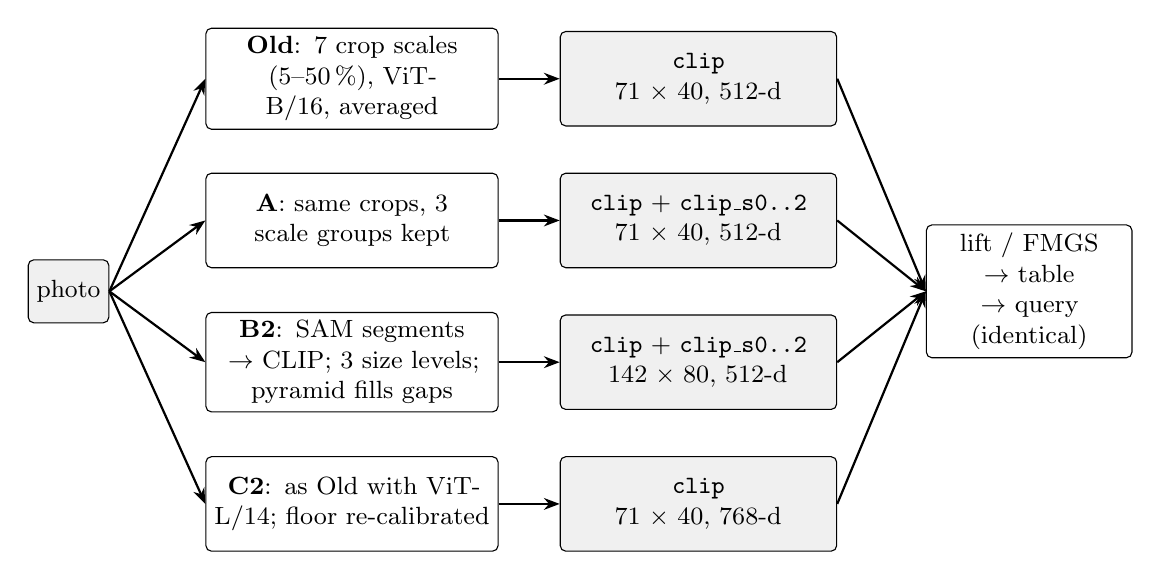
\begin{tikzpicture}[font=\small,
   w/.style={box, text width=3.5cm, minimum height=12mm},
   o/.style={data, text width=3.3cm, minimum height=12mm}]
  \node[data] (img) at (0,0) {photo};
  \node[w] (o1) at (3.6,2.7) {\textbf{Old}: 7 crop scales (5--50\,\%), ViT-B/16, averaged};
  \node[w] (a1) at (3.6,0.9) {\textbf{A}: same crops, 3 scale groups kept};
  \node[w] (b1) at (3.6,-0.9) {\textbf{B2}: SAM segments $\rightarrow$ CLIP; 3 size levels; pyramid fills gaps};
  \node[w] (c1) at (3.6,-2.7) {\textbf{C2}: as Old with ViT-L/14; floor re-calibrated};
  \node[o] (o2) at (8.0,2.7) {\code{clip}\\$71\times40$, 512-d};
  \node[o] (a2) at (8.0,0.9) {\code{clip} + \code{clip\_s0..2}\\$71\times40$, 512-d};
  \node[o] (b2) at (8.0,-0.9) {\code{clip} + \code{clip\_s0..2}\\$142\times80$, 512-d};
  \node[o] (c2) at (8.0,-2.7) {\code{clip}\\$71\times40$, 768-d};
  \node[box, text width=2.4cm] (rest) at (12.2,0) {lift / FMGS\\$\rightarrow$ table\\$\rightarrow$ query\\(identical)};
  \foreach \n in {o,a,b,c} {\draw[arr] (img.east) -- (\n1.west); \draw[arr] (\n1) -- (\n2); \draw[arr] (\n2.east) -- (rest.west);}
\end{tikzpicture}
\caption{The four CLIP teacher designs. Grids are per photo for a $16{:}9$ image (cell size 2.5\,\% of the short side;
B2 uses 1.25\,\%). DINOv2 is the same in all designs.}
\label{fig:teachers}
\end{figure}

\subsection{Old: the scale-averaged crop pyramid (LERF/FMGS style)}
OpenCLIP ViT-B/16 (LAION-2B, \code{laion2b\_s34b\_b88k}, 512-d). For each of seven scales
$s\in\{0.05, 0.125, 0.2, 0.275, 0.35, 0.425, 0.5\}$ of the photo's short side, square crops of side
$s\cdot\min(H,W)$ (at least 16\,px) slide with half-crop stride; each is resized to $224\times224$ and embedded to a unit
vector placed at the crop centre. Each scale's grid is resampled onto the common grid (cell = 2.5\,\% of the short
side, $\approx71\times40$) and the seven scales are \textbf{averaged with equal weight}, as FMGS does. About 3{,}500 crops
per frame (1.06\,M for backroom); 31\,min for backroom and 53\,min for flightroom; 1.3 / 2.2\,GB of fp16 maps.

\subsection{A: multi-scale, scale chosen per query (merged 8 Oct)}
\textbf{Motivation.} A diagnostic (Section~\ref{sec:diag}) showed that averaging costs 0.07--0.09 relevancy: a 5\,\% crop
around a small object is averaged with crops covering half the image. LERF instead keeps scales separate and picks one
per query.\\
\textbf{How.} The same seven scales, grouped into \emph{small} ($s<0.15$: 0.05, 0.125), \emph{medium}
($0.15\le s<0.4$: 0.2, 0.275, 0.35) and \emph{large} ($s\ge0.4$: 0.425, 0.5); each group averaged on its own and stored as
\code{clip\_s0..2}, plus the overall average \code{clip}. Same crops, so the same teacher time; maps 3.8 / 6.4\,GB.
The lift lifts each group separately (the overall mean follows by linearity); the table carries a
\code{clip\_scales} block ($n\times3\times512$). At query time relevancy is computed per group and the group whose top-100
relevancies peak highest is used (LERF's rule). For FMGS the field gets one CLIP head per group, and each training step
trains one randomly chosen group.

\subsection{B and B2: region-level CLIP from SAM segments}
\textbf{Motivation.} Give CLIP whole objects rather than square windows that mix an object with its surroundings
(LangSplat's idea).\\
\textbf{B.} SAM ViT-B's automatic mask generator ($32\times32$ prompt points; segments below 0.05\,\% of the image
dropped) segments each photo. Each segment is cut out --- its bounding box plus 10\,\% context, pixels outside the mask
blacked out, padded to a square, resized to 224 --- and embedded with CLIP. Each cell of a two-times finer grid
(1.25\,\% cells, $\approx142\times80$) gets the coverage-weighted mean of the unit embeddings of the segments covering it.
Cells no segment covers stay \textbf{zero}.\\
\textbf{What went wrong with B} (lift 19/29, F-C 9/29, FMGS collapsed on flightroom with 15/16 ``no candidate''): the
lift ignores zero cells (they add nothing to the weighted sum), but FMGS learns them as targets; thin structures (PVC
frame, round table) yield poor segments.\\
\textbf{B2} keeps B's segment embeddings and adds three things:
\begin{enumerate}
  \item \textbf{Pyramid fallback.} Every cell no segment covers takes that photo's Old pyramid feature (read from the
        Old teacher cache, resampled to the finer grid), so no zero vectors remain.
  \item \textbf{Size levels.} Segments are split by area into \emph{parts} ($<1\,\%$ of the image), \emph{objects}
        (1--10\,\%) and \emph{regions} ($\ge10\,\%$), painted into three maps \code{clip\_s0..2} (uncovered cells again
        from the pyramid). The query picks the level with the highest peak exactly as A picks a scale; the
        \code{clip} map paints all segments together and is what the \emph{flat} variant uses.
  \item \textbf{Mask cache.} SAM masks are stored per photo (bit-packed, 18 / 14\,MB), so later SAM builds skip
        segmentation.
\end{enumerate}
Cost: 41 / 47\,min of teachers (24{,}732 / 28{,}690 segment crops instead of $\approx$1\,M square crops); maps
13.8 / 23.0\,GB (finer grid $\times$ four maps).

\begin{figure}[ht]
\centering
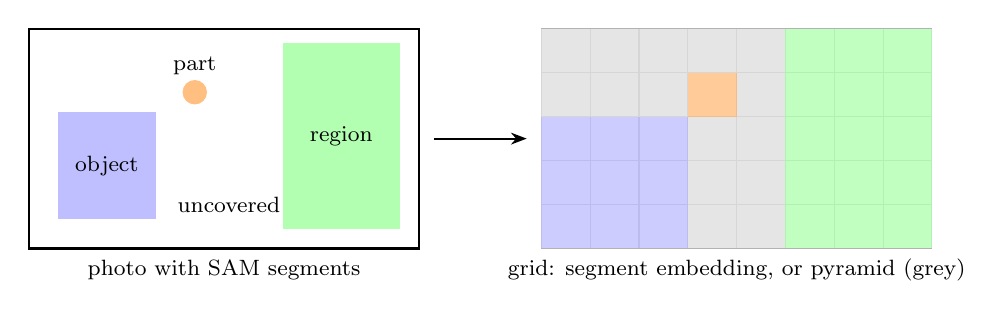
\begin{tikzpicture}[scale=0.62, font=\footnotesize]
  \draw[thick] (0,0) rectangle (8,4.5); \node at (4,-0.45) {photo with SAM segments};
  \fill[blue!25] (0.6,0.6) rectangle (2.6,2.8); \node at (1.6,1.7) {object};
  \fill[green!30] (5.2,0.4) -- (7.6,0.4) -- (7.6,4.2) -- (5.2,4.2) -- cycle; \node at (6.4,2.3) {region};
  \fill[orange!50] (3.4,3.2) circle (0.25); \node at (3.4,3.75) {part};
  \node[align=center] at (4.1,0.9) {uncovered};
  \begin{scope}[xshift=10.5cm]
    \foreach \x in {0,...,7} \foreach \y in {0,...,4} \draw[gray!60] (\x,\y*0.9) rectangle ++(1,0.9);
    \fill[blue!25, opacity=0.8] (0,0) rectangle (3,2.7);
    \fill[green!30, opacity=0.8] (5,0) rectangle (8,4.5);
    \fill[orange!50, opacity=0.8] (3,2.7) rectangle (4,3.6);
    \fill[gray!25, opacity=0.8] (3,0) rectangle (5,2.7); \fill[gray!25, opacity=0.8] (0,2.7) rectangle (3,4.5);
    \fill[gray!25, opacity=0.8] (4,2.7) rectangle (5,4.5); \fill[gray!25, opacity=0.8] (3,3.6) rectangle (4,4.5);
    \node at (4,-0.45) {grid: segment embedding, or pyramid (grey)};
  \end{scope}
  \draw[arr] (8.3,2.25) -- (10.2,2.25);
\end{tikzpicture}
\caption{B2's grid: cells covered by a segment take the coverage-weighted segment embedding; uncovered cells (grey) take
the pyramid feature. Segments are also split into part / object / region levels, one map each.}
\end{figure}

\subsection{C and C2: a larger CLIP}
\textbf{C.} The Old pyramid with OpenCLIP ViT-L/14 (\code{laion2b\_s32b\_b82k}, 768-d); the query encodes text with the
same model. Teachers take 216 / 363\,min (6--7$\times$ Old), maps 1.75 / 2.9\,GB. C scored 18/29 on the lift ---
but the query's floor (0.55) had been fixed on ViT-B/16, and relevancy is a sigmoid of similarity \emph{differences}
whose scale depends on the model.\\
\textbf{C2} calibrates the floor without using any evaluation query (\code{scripts/calibrate\_floor.py}). For a neutral
vocabulary of 30 everyday objects that appear in no development or Phase~5 query (laptop, printer, ladder, helmet,
\dots), it computes on each scene the fraction $q$ of Gaussians whose Old relevancy is below 0.55, pooled over all words,
and takes the ViT-L/14 relevancy at the same quantile $q$. The mean over scenes, \textbf{0.5222} (backroom 0.498,
flightroom 0.546), is written into the C tables' \code{index.json}; the query uses a table's own floor when one is
present. The tables are those of C; only the query changes.

%=======================================================================================
\section{Attaching features to the Gaussians}
%=======================================================================================

\subsection{The lift (training-free)}
For Gaussian $i$, teacher map $F_v$ of view $v$ (bilinearly upsampled to the render size, 960\,px wide) and its blend
weight $w_i(v,p)$ at pixel $p$:
\begin{equation}
  \vect{f}_i = \frac{\sum_{v,p} w_i(v,p)\,F_v(p)}{\sum_{v,p} w_i(v,p)} .
\end{equation}
Rendering is linear in the per-Gaussian features, so the numerator is the gradient of
$\sum_p\langle\mathrm{render}(\vect{f}),F_v\rangle$ at $\vect{f}=0$ and the denominator the gradient of
$\sum_p\mathrm{render}(\vect{1})$: two backward passes per view and chunk, no optimisation (Phase~0 verified the
identities numerically). Gaussians with total weight 0 are \emph{unseen} and score 0 at query time.

\textbf{With scale groups (A, B2)} the lift accumulates \code{dino} and the three \code{clip\_s*} maps; \code{clip} is
their mean by linearity. The accumulators ($n\times(384+3\cdot512)$ floats) live in host RAM, which is why the lift's GPU
peak falls from 7.4 to 0.8\,GB while its time rises from 3--4 to 15--23\,min (more chunks, host transfers).

\subsection{FMGS (trained feature field)}
\begin{figure}[ht]
\centering
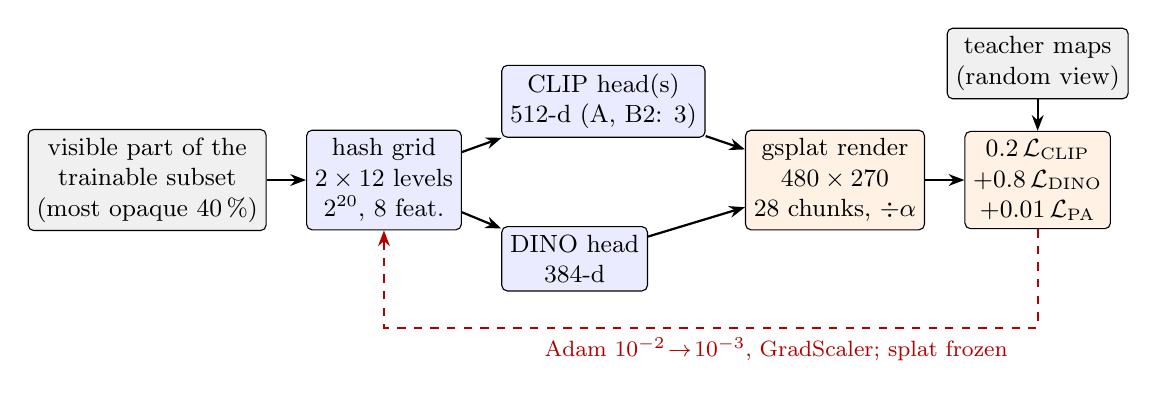
\begin{tikzpicture}[node distance=4mm and 5mm, font=\small]
  \node[data] (sub) {visible part of the\\trainable subset\\(most opaque 40\,\%)};
  \node[model, right=of sub] (hg) {hash grid\\$2\times12$ levels\\$2^{20}$, 8 feat.};
  \node[model, right=of hg, yshift=10mm] (hc) {CLIP head(s)\\512-d (A, B2: 3)};
  \node[model, right=of hg, yshift=-10mm] (hd) {DINO head\\384-d};
  \node[stp, right=of hc, yshift=-10mm] (rend) {gsplat render\\$480\times270$\\28 chunks, $\div\alpha$};
  \node[stp, right=of rend] (loss) {$0.2\,\mathcal{L}_\mathrm{CLIP}$\\$+0.8\,\mathcal{L}_\mathrm{DINO}$\\$+0.01\,\mathcal{L}_\mathrm{PA}$};
  \node[data, above=of loss] (tm) {teacher maps\\(random view)};
  \draw[arr] (sub) -- (hg); \draw[arr] (hg) -- (hc); \draw[arr] (hg) -- (hd);
  \draw[arr] (hc) -- (rend); \draw[arr] (hd) -- (rend); \draw[arr] (rend) -- (loss); \draw[arr] (tm) -- (loss);
  \draw[arr, dashed, red!70!black] (loss.south) -- ++(0,-1.25) -| node[pos=0.2, below, font=\footnotesize]
     {Adam $10^{-2}\!\to\!10^{-3}$, GradScaler; splat frozen} (hg.south);
\end{tikzpicture}
\caption{One FMGS training step (4{,}200 steps). F-C uses only $\mathcal{L}_\mathrm{CLIP}$.}
\end{figure}

\begin{itemize}
  \item \textbf{Field.} Centres are normalised into the scene's 1st--99th percentile box (padded 5\,\%) and encoded by
        a 24-level hash grid (16 $\rightarrow$ 512, $2^{20}$ entries, 8 features per level = 192-d) followed by MLP heads
        (2 hidden layers of 256), all tiny-cuda-nn in fp16; 113.5\,M parameters. On sm\_75 a 192-d grid will not launch,
        so the 24 levels are built as two consecutive 12-level grids (16$\rightarrow$84, 98$\rightarrow$512; every
        level within 1\,\% of the single ladder) --- a reported deviation.
  \item \textbf{Each step}: a random training view; the trainable subset (the most opaque 40\,\% of Gaussians, chosen
        once) restricted to those projecting into the view; field evaluated at their centres; features rendered at
        $480\times270$ and divided by rendered alpha; loss on pixels with alpha $\ge0.5$:
        $\mathcal{L}_\mathrm{CLIP}$ Huber ($\delta=1.25$), $\mathcal{L}_\mathrm{DINO}$ squared error, and pixel
        alignment $\mathcal{L}_\mathrm{PA}=\mathrm{mean}\,|\cos(\hat c_p,\hat c_q)-\cos(d_p,d_q)|$ over 4{,}096 sampled
        pixels and their $3\times3$ neighbours at dilation 2.
  \item \textbf{Memory and precision} (Phase~4): expandable segments for PyTorch's allocator, tiny-cuda-nn's OOM
        recognised with one retry per step, dynamic loss scaling (the CLIP term's fp16 gradients underflowed), and a
        $10^{-3}$ norm floor in pixel alignment. Typical run: 30\,min, peak 7.8\,GB device; F-C 11--14\,min.
  \item \textbf{Variants.} A and B2: one CLIP head per scale group / size level, one group trained per step.
        C: 768-d heads did not fit tiny-cuda-nn's memory and fell back to PyTorch heads (slower: F-CD 43 / 34\,min).
  \item \textbf{Bake}: the field is evaluated at all centres, rows unit-normalised, unseen rows (from the lift's blend
        weights) marked; the field is kept (\code{field.pt}).
\end{itemize}

%=======================================================================================
\section{The table and the query}
%=======================================================================================

\paragraph{Table.} Raw little-endian arrays per run and checkpoint: \code{clip.f16} ($n\times512$ or 768),
\code{clip\_\-scales.f16} ($n\times3\times512$, A and B2), \code{dino.f16}, \code{weight.f32} (0 = unseen),
\code{geom.f32} (centre, opacity, largest scale), \code{pca\_rgb.u8} and \code{index.json} (key, CLIP model, settings,
build metrics, optional calibrated floor). Row $i$ is record $i$ of Galley's \code{.splat}; a hash of that ordering is
checked so a stale table can never colour the wrong Gaussians.

\begin{figure}[ht]
\centering
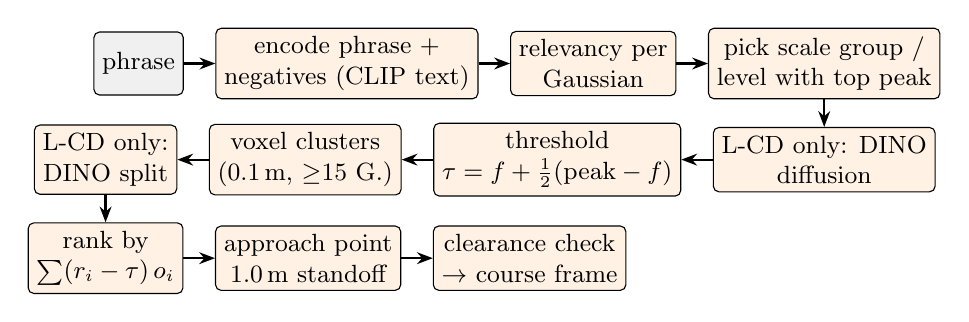
\begin{tikzpicture}[node distance=3.5mm and 4mm, font=\small]
  \node[data] (t) {phrase};
  \node[stp, right=of t] (e) {encode phrase +\\negatives (CLIP text)};
  \node[stp, right=of e] (r) {relevancy per\\Gaussian};
  \node[stp, right=of r] (g) {pick scale group /\\level with top peak};
  \node[stp, below=of g] (d) {L-CD only: DINO\\diffusion};
  \node[stp, left=of d] (th) {threshold\\$\tau=f+\tfrac12(\mathrm{peak}-f)$};
  \node[stp, left=of th] (cl) {voxel clusters\\(0.1\,m, $\ge$15 G.)};
  \node[stp, left=of cl] (sp) {L-CD only:\\DINO split};
  \node[stp, below=of sp] (rk) {rank by\\$\sum(r_i-\tau)\,o_i$};
  \node[stp, right=of rk] (ap) {approach point\\1.0\,m standoff};
  \node[stp, right=of ap] (cl2) {clearance check\\$\rightarrow$ course frame};
  \draw[arr] (t) -- (e); \draw[arr] (e) -- (r); \draw[arr] (r) -- (g); \draw[arr] (g) -- (d);
  \draw[arr] (d) -- (th); \draw[arr] (th) -- (cl); \draw[arr] (cl) -- (sp); \draw[arr] (sp) -- (rk);
  \draw[arr] (rk) -- (ap); \draw[arr] (ap) -- (cl2);
\end{tikzpicture}
\caption{The query. $f$ is the floor (0.55; C2: 0.5222). The group choice applies only to tables with
\code{clip\_scales} (A, B2) and is skipped in the \emph{flat} variants.}
\label{fig:query}
\end{figure}

\paragraph{Query steps} (Figure~\ref{fig:query}; CPU worker, table memory-mapped).
\begin{enumerate}
  \item \textbf{Relevancy} (LERF): $r_i=\min_j\sigma\bigl(10\,(\cos(\vect f_i,\vect t)-\cos(\vect f_i,\vect n_j))\bigr)$
        with negatives \emph{object, things, stuff, texture}; unseen Gaussians get 0.
  \item \textbf{Scale / level choice} (A, B2): relevancy per group; the group with the highest peak wins.
  \item \textbf{Peak and threshold}: peak = mean of the top 100 relevancies among Gaussians with opacity $\ge0.1$;
        $\tau = f + 0.5\,(\mathrm{peak}-f)$ (a fixed $\tau$ let every white wall into ``whiteboard''). Keep
        $r_i\ge\tau$, opacity $\ge0.1$.
  \item \textbf{L-CD diffusion}: relevancy smoothed twice over each Gaussian's 16 nearest neighbours, edges weighted by
        clipped DINO cosine ($r\leftarrow0.5\,r+0.5\cdot$weighted neighbour mean).
  \item \textbf{Clusters}: connected components on a 0.1\,m voxel grid (26-neighbourhood); clusters of fewer than 15
        Gaussians are dropped. \textbf{L-CD split}: a cluster whose DINO rows form two groups with mean-direction cosine
        $<0.5$ (spherical 2-means) becomes two candidates.
  \item \textbf{Rank} by $\sum(r_i-\tau)\,o_i$; report centroid, 5--95\,\% box, margin to the runner-up (ambiguous if
        $<0.25$).
  \item \textbf{Approach point} 1.0\,m from the centroid, horizontally towards the cameras that looked at it, inside
        the flyable box; clearance = 5th-nearest sparse SfM point minus the 0.19\,m body radius (gap $<0.15$\,m flagged);
        converted to the course frame $(x,-y,-z)$.
\end{enumerate}

\begin{figure}[ht]
\centering
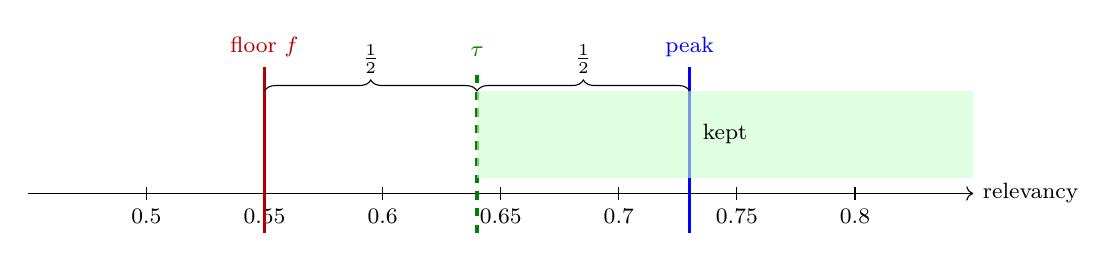
\begin{tikzpicture}[xscale=30, yscale=1, font=\footnotesize]
  \draw[->] (0.45,0) -- (0.85,0) node[right] {relevancy};
  \foreach \x in {0.5,0.55,0.6,0.65,0.7,0.75,0.8} \draw (\x,0.08) -- (\x,-0.08) node[below] {\x};
  \draw[very thick, red!70!black] (0.55,-0.5) -- (0.55,1.6) node[above] {floor $f$};
  \draw[very thick, blue] (0.73,-0.5) -- (0.73,1.6) node[above] {peak};
  \draw[very thick, green!50!black, dashed] (0.64,-0.5) -- (0.64,1.6) node[above] {$\tau$};
  \fill[green!20, opacity=0.6] (0.64,0.2) rectangle (0.85,1.3); \node at (0.745,0.75) {kept};
  \draw[decorate, decoration={brace, amplitude=4pt}] (0.55,1.3) -- (0.64,1.3) node[midway, above=3pt] {$\tfrac12$};
  \draw[decorate, decoration={brace, amplitude=4pt}] (0.64,1.3) -- (0.73,1.3) node[midway, above=3pt] {$\tfrac12$};
\end{tikzpicture}
\caption{The relative threshold: halfway between the floor and the query's own peak. If the peak is below the floor,
$\tau=f$ and nothing usually survives (``no candidate''). Raising every relevancy by a constant has the same effect as
lowering the floor --- the key to Section~\ref{sec:floor}.}
\label{fig:tau}
\end{figure}

%=======================================================================================
\section{Evaluation protocol}
%=======================================================================================

\begin{itemize}
  \item \textbf{Query sets} were written and annotated \emph{before} any result was seen (frozen in commit
        \code{f38225b}): backroom 13 present objects + 3 absent (bicycle, sofa, ceiling fan); flightroom 16 + 3 (red tool
        chest, recycling bin, bicycle). Objects with several copies are annotated as instances. The five Phase~1 queries
        that shaped the threshold are a separate development set and are not used here.
  \item \textbf{Amended sets} (7~Oct): a ground-truth check found two of our own annotation errors (purple foam mat
        placed on points behind it; glass door cabinet missing its upper instances); both were re-placed from the
        splat's rendered depth independently of any model output. The originals are kept; all results here use the
        amended sets.
  \item \textbf{Hit}: the top candidate's box grown by 0.3\,m contains an annotated instance, or its centroid is within
        0.75\,m of one. \textbf{Error}: centroid to nearest instance. \textbf{Failures}: \emph{no candidate};
        \emph{bad position} (top centroid within 1.5\,m of an instance); \emph{wrong object}.
  \item \textbf{Absent objects}: \emph{neg.\ FP} = fraction producing any candidate; \emph{AUROC} = probability that a
        present object's peak exceeds an absent object's (threshold-free).
  \item Query settings are the defaults throughout, never tuned on these sets; the floor sweep
        (Section~\ref{sec:floor}) is explicitly a post-hoc analysis.
\end{itemize}

%=======================================================================================
\section{Results}
%=======================================================================================

\begin{table}[ht]
\centering\small
\begin{tabular}{@{}lcccc@{}}
\toprule
 & \multicolumn{4}{c}{Top-1 hits: backroom /13 + flightroom /16 = total /29} \\
\cmidrule(l){2-5}
Teachers & Lift L-C & Lift L-CD & FMGS F-C & FMGS F-CD \\
\midrule
Old (averaged pyramid)            & 10+10 = 20 & 10+10 = 20 & 7+8 = \textbf{15} & 7+4 = \textbf{11} \\
\textbf{A} multi-scale (default)  & 9+13 = \textbf{22} & 10+12 = \textbf{22} & 7+8 = \textbf{15} & 4+4 = 8 \\
\textbf{B2} SAM levels + fallback & 9+12 = 21 & 10+11 = 21 & 6+6 = 12 & 3+3 = 6 \\
\quad B2 flat (no level choice)   & 10+11 = 21 & --- & 7+4 = 11 & --- \\
\textbf{C2} ViT-L/14, calibrated  & 8+11 = 19 & 8+10 = 18 & 4+6 = 10 & 3+2 = 5 \\
\midrule
\textit{B} (first SAM version)    & \textit{8+11 = 19} & \textit{8+7 = 15} & \textit{8+1 = 9} & \textit{6+0 = 6} \\
\textit{C} (ViT-L/14, floor 0.55) & \textit{8+10 = 18} & \textit{8+9 = 17} & \textit{4+4 = 8} & \textit{3+1 = 4} \\
\bottomrule
\end{tabular}
\caption{Main result at the default query settings, amended query sets.}
\label{tab:main}
\end{table}

\begin{figure}[ht]
\centering
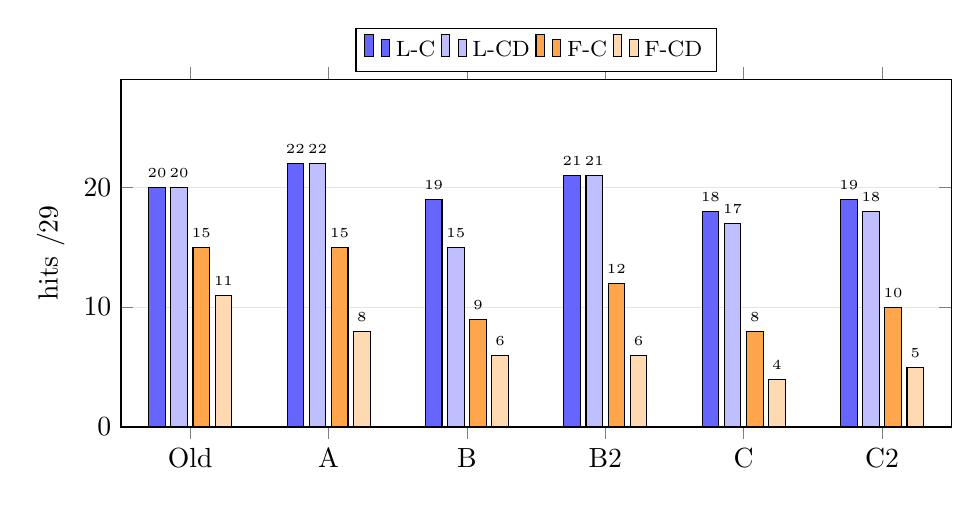
\begin{tikzpicture}
\begin{axis}[ybar, bar width=6pt, width=\linewidth, height=6cm, ymin=0, ymax=29, ylabel={hits /29},
  symbolic x coords={Old,A,B,B2,C,C2}, xtick=data, enlarge x limits=0.1,
  legend style={at={(0.5,1.02)}, anchor=south, legend columns=4, font=\footnotesize},
  nodes near coords, every node near coord/.append style={font=\tiny}, ymajorgrids, grid style={gray!20}]
  \addplot[fill=blue!60] coordinates {(Old,20) (A,22) (B,19) (B2,21) (C,18) (C2,19)};
  \addplot[fill=blue!25] coordinates {(Old,20) (A,22) (B,15) (B2,21) (C,17) (C2,18)};
  \addplot[fill=orange!70] coordinates {(Old,15) (A,15) (B,9) (B2,12) (C,8) (C2,10)};
  \addplot[fill=orange!30] coordinates {(Old,11) (A,8) (B,6) (B2,6) (C,4) (C2,5)};
  \legend{L-C, L-CD, F-C, F-CD}
\end{axis}
\end{tikzpicture}
\caption{Hits per teacher design and backend (default settings). The lift beats FMGS for every design.}
\label{fig:bars}
\end{figure}

\begin{table}[ht]
\centering\small
\begin{tabularx}{\linewidth}{@{}Lcccccc@{}}
\toprule
Lift L-C (backroom / flightroom) & Median err.\ (m) & Neg.\ FP & AUROC & Lift (min) & Table (GB) & Query (s) \\
\midrule
Old & 0.19 / 0.22 & 1/3, 1/3 & 0.85 / 0.90 & 3.0 / 4.4 & 0.92 / 0.66 & 0.78 / 0.54 \\
A   & 0.21 / 0.25 & 1/3, 1/3 & 0.87 / 0.90 & 17.4 / 22.6 & 2.48 / 1.77 & 2.70 / 1.96 \\
B2  & 0.19 / 0.20 & 1/3, 1/3 & 0.87 / 0.94 & 14.7 / 16.8 & 2.48 / 1.77 & 2.67 / 1.94 \\
B2 flat & 0.17 / 0.19 & 1/3, 0 & 0.87 / 0.94 & 14.7 / 16.8 & 2.48 / 1.77 & 0.71 / 0.53 \\
C2  & 0.16 / 0.27 & 1/3, 0 & 0.77 / 0.96 & 3.7 / 5.4 & 1.18 / 0.84 & 1.45 / 0.90 \\
\bottomrule
\end{tabularx}
\caption{Lift quality and cost. Median error over the candidates returned (hits and misses). Query time is the
evaluation's median on the CPU (A and B2 compute four relevancy maps per query).}
\label{tab:liftdetail}
\end{table}

\begin{table}[ht]
\centering\small
\begin{tabular}{@{}lcccccc@{}}
\toprule
\shortstack[l]{Build\\(backroom / flightroom)} & \shortstack{Teachers\\(min)} & \shortstack{Teacher\\maps (GB)} & \shortstack{Lift\\(min)} & \shortstack{F-C\\(min)} & \shortstack{F-CD\\(min)} & \shortstack{Lift peak\\VRAM (GB)} \\
\midrule
Old & 31 / 53   & 1.3 / 2.2   & 3.0 / 4.4   & 13.9 / 11.5 & 31.4 / 25.2 & 7.4 / 2.4 \\
A   & 32 / 53   & 3.8 / 6.4   & 17.4 / 22.6 & 13.6 / 11.4 & 30.6 / 25.2 & 0.8 / 0.8 \\
B2  & 41 / 47   & 13.8 / 23.0 & 14.7 / 16.8 & 13.6 / 11.3 & 30.3 / 25.2 & 0.8 / 0.8 \\
C2  & 216 / 363 & 1.8 / 2.9   & 3.7 / 5.4   & 21.7 / 17.5 & 43.2 / 34.3 & 4.6 / 2.4 \\
\bottomrule
\end{tabular}
\caption{Build cost on the RTX~2080 (8\,GB). Teachers are shared by all backends of a design. B2 reuses Old's pyramid
cache for its fallback; C2 reuses C's tables.}
\end{table}

\FloatBarrier
\subsection{Per query}

\begin{table}[ht]
\centering\footnotesize
\setlength{\tabcolsep}{2pt}
\begin{tabular}{@{}l*{5}{C}|*{4}{C}|*{4}{C}|*{4}{C}@{}}
\toprule
 & \multicolumn{5}{c|}{L-C} & \multicolumn{4}{c|}{L-CD} & \multicolumn{4}{c|}{F-C} & \multicolumn{4}{c}{F-CD} \\
Query & Old & A & B2 & B2f & C2 & Old & A & B2 & C2 & Old & A & B2 & C2 & Old & A & B2 & C2 \\
\midrule
\multicolumn{18}{@{}l}{\emph{backroom}} \\
recycling bin & \Y&\Y&\Y&\Y&\Y & \Y&\Y&\Y&\Y & \Y&\Y&\Y&\Y & \Y&\Y&\Y&\Y \\
blue trash can & \Y&\Y&\Y&\Y&\Y & \Y&\Y&\Y&\Y & \Y&\Y&\Y&\Y & \Y&\Y&\Y&\Y \\
office chair & \Y&\Y&\Y&\Y&\N & \Y&\Y&\Y&\N & \B&\B&\N&\N & \Y&\B&\N&\N \\
swivel chair & \N&\B&\N&\N&\N & \N&\Y&\N&\N & \B&\B&\N&\N & \N&\N&\N&\N \\
grandfather clock & \Y&\Y&\Y&\Y&\Y & \Y&\Y&\Y&\Y & \Y&\Y&\Y&\N & \Y&\N&\N&\B \\
clock & \Y&\Y&\Y&\Y&\Y & \Y&\Y&\Y&\Y & \Y&\Y&\Y&\N & \N&\N&\N&\N \\
children's road play mat & \Y&\Y&\Y&\Y&\Y & \Y&\Y&\Y&\Y & \Y&\Y&\Y&\Y & \Y&\W&\Y&\N \\
camera tripod & \N&\N&\N&\N&\N & \N&\N&\N&\N & \N&\N&\N&\N & \N&\N&\N&\N \\
purple foam mat & \Y&\Y&\Y&\Y&\W & \Y&\Y&\Y&\W & \Y&\W&\W&\W & \W&\W&\B&\W \\
white bucket & \W&\W&\W&\W&\W & \W&\W&\W&\W & \N&\N&\N&\N & \N&\N&\N&\N \\
glass door cabinet & \Y&\Y&\Y&\Y&\Y & \Y&\Y&\Y&\Y & \B&\Y&\Y&\N & \Y&\Y&\N&\W \\
hose reel & \Y&\W&\W&\Y&\Y & \Y&\W&\Y&\Y & \W&\W&\W&\N & \N&\W&\N&\N \\
moving box & \Y&\Y&\Y&\Y&\Y & \Y&\Y&\Y&\Y & \Y&\Y&\W&\Y & \Y&\Y&\W&\Y \\
\multicolumn{18}{@{}l}{\emph{flightroom}} \\
armchair & \N&\Y&\Y&\Y&\Y & \N&\Y&\Y&\N & \N&\N&\N&\N & \N&\N&\N&\N \\
upholstered chair & \N&\Y&\Y&\N&\N & \N&\Y&\N&\N & \N&\N&\N&\N & \N&\N&\N&\N \\
whiteboard & \Y&\Y&\Y&\Y&\Y & \Y&\Y&\Y&\Y & \Y&\Y&\Y&\Y & \Y&\Y&\Y&\Y \\
computer monitor & \Y&\Y&\Y&\Y&\Y & \Y&\Y&\Y&\Y & \Y&\Y&\Y&\Y & \Y&\W&\N&\W \\
keyboard & \N&\N&\N&\N&\N & \N&\N&\N&\N & \N&\N&\N&\N & \N&\N&\N&\N \\
floor lamp & \N&\N&\N&\N&\N & \N&\N&\N&\N & \W&\N&\N&\N & \N&\N&\N&\N \\
red cup & \Y&\Y&\Y&\Y&\Y & \Y&\Y&\Y&\Y & \Y&\Y&\N&\Y & \N&\N&\N&\N \\
water bottle & \Y&\Y&\Y&\Y&\Y & \Y&\Y&\Y&\Y & \Y&\N&\N&\Y & \N&\N&\N&\N \\
water jug & \B&\Y&\B&\B&\B & \B&\B&\B&\B & \W&\N&\N&\N & \N&\N&\N&\N \\
round table & \Y&\Y&\Y&\Y&\Y & \Y&\Y&\Y&\Y & \W&\Y&\N&\W & \N&\N&\N&\N \\
drone gate & \W&\W&\W&\W&\W & \W&\W&\W&\N & \W&\W&\N&\N & \N&\W&\N&\N \\
PVC pipe frame & \Y&\Y&\Y&\Y&\Y & \Y&\Y&\Y&\Y & \Y&\Y&\Y&\Y & \Y&\Y&\Y&\Y \\
poster & \Y&\Y&\Y&\Y&\Y & \Y&\Y&\Y&\Y & \Y&\Y&\Y&\Y & \Y&\Y&\Y&\B \\
garden cart & \Y&\Y&\Y&\Y&\Y & \Y&\Y&\Y&\Y & \Y&\Y&\Y&\N & \N&\N&\N&\N \\
wheelbarrow & \Y&\Y&\Y&\Y&\Y & \Y&\Y&\Y&\Y & \Y&\Y&\Y&\N & \N&\Y&\N&\N \\
cardboard box & \Y&\Y&\Y&\Y&\Y & \Y&\Y&\Y&\Y & \N&\N&\N&\N & \N&\N&\N&\N \\
\midrule
hits /29 & 20&22&21&21&19 & 20&22&21&18 & 15&15&12&10 & 11&8&6&5 \\
\bottomrule
\end{tabular}
\caption{Outcome per query. \textbf{H} hit; n no candidate; b bad position (right area, $>$0.75\,m off); w wrong object.
B2f = B2 flat.}
\label{tab:perquery}
\end{table}

\paragraph{What changes between designs (lift L-C, versus Old).}
\begin{itemize}
  \item \textbf{A}: +armchair, +upholstered chair, +water jug; $-$hose reel (net +2).
  \item \textbf{B2}: +armchair, +upholstered chair; $-$hose reel (net +1). B2 flat: +armchair (net +1).
  \item \textbf{C2}: +armchair; $-$office chair, $-$purple foam mat (net $-$1).
  \item Union over every design and lift variant: 24/29 (A's L-CD adds swivel chair; Old, B2 flat and C2 keep hose reel).
        \textbf{Missed by everything}: camera tripod, white bucket, keyboard, floor lamp, drone gate.
\end{itemize}

%=======================================================================================
\section{Why: analysis of the observations}
%=======================================================================================

\subsection{Where the signal is lost (diagnostic, 7 Oct)}
\label{sec:diag}
For every annotated object, the three nearest training photos showing it were used to measure the Old relevancy at
three stages: (a) on the cached teacher grid at the object's pixel; (d) on CLIP crops \emph{centred} on the object at
each of the seven scales (best kept); (c) in the lifted table, at Gaussians within 0.25\,m of the annotation.

\begin{table}[ht]
\centering\small
\begin{tabular}{@{}lccc@{}}
\toprule
Group (Old, L-C) & (a) teacher grid & (d) best centred scale & (c) 3D table \\
\midrule
hits (18)               & 0.682 & 0.748 (+0.066) & 0.675 ($-$0.007) \\
misses (11)             & 0.485 & 0.577 (+0.093) & 0.517 \\
no-candidate misses (6) & 0.439 & 0.522 (+0.083) & 0.504 \\
\bottomrule
\end{tabular}
\caption{Mean relevancy at each stage (0.5 = indifferent, floor 0.55).}
\end{table}

\textbf{Lifting into 3D loses almost nothing} ($-0.007$); the loss happens in 2D. Scale averaging costs 0.07--0.09
everywhere; large objects peak at the 0.5 scale and small ones at 0.05--0.2, so no fixed scale suits all. Some misses are
\emph{recognition} limits: keyboard (0.50), floor lamp (0.52) and armchair (0.40) stay low even on a centred crop at the
best scale.

\subsection{A's gain at the default floor is mostly a floor effect}
\label{sec:floor}
A takes, per query, the \emph{maximum} over three groups of the top-100 mean relevancy. A maximum of three noisy
estimates is higher than their average --- for absent objects as much as for present ones (Figure~\ref{fig:scatter}):
the mean peak of present objects rises from 0.624 to 0.679 and that of absent objects from 0.511 to 0.547. With the floor
fixed at 0.55, this behaves like lowering the floor by $\approx$0.045 (Figure~\ref{fig:tau}).

\begin{figure}[ht]
\centering
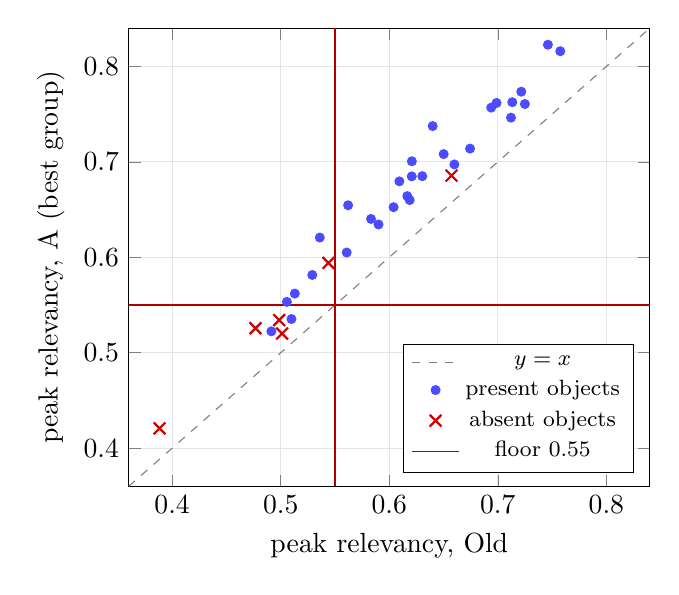
\begin{tikzpicture}
\begin{axis}[width=8.2cm, height=7.4cm, xmin=0.36, xmax=0.84, ymin=0.36, ymax=0.84,
  xlabel={peak relevancy, Old}, ylabel={peak relevancy, A (best group)},
  legend pos=south east, legend style={font=\footnotesize}, grid=major, grid style={gray!20}]
  \addplot[gray, dashed, domain=0.36:0.84] {x}; \addlegendentry{$y=x$}
\addplot[only marks, mark=*, mark size=1.6pt, blue!70] coordinates {(0.7216,0.7735) (0.6939,0.7568) (0.5621,0.6545) (0.536,0.6207) (0.6744,0.7139) (0.66,0.6973) (0.7575,0.8159) (0.5099,0.5353) (0.7249,0.7606) (0.5608,0.605) (0.6501,0.7081) (0.6304,0.685) (0.6988,0.7617) (0.5291,0.5815) (0.5057,0.5533) (0.7133,0.7625) (0.6166,0.6641) (0.4914,0.5224) (0.513,0.562) (0.7121,0.7463) (0.604,0.6525) (0.5901,0.6344) (0.5832,0.6402) (0.6093,0.6796) (0.7461,0.8227) (0.64,0.7375) (0.6208,0.7006) (0.6207,0.6848) (0.6188,0.66)};
\addlegendentry{present objects}
\addplot[only marks, mark=x, mark size=3pt, red!80!black, thick] coordinates {(0.4986,0.5342) (0.3884,0.4208) (0.6573,0.6856) (0.5013,0.5201) (0.544,0.5941) (0.4768,0.5257)};
\addlegendentry{absent objects}

  \addplot[red!70!black, thin, domain=0.36:0.84] {0.55}; \addlegendentry{floor 0.55}
  \addplot[red!70!black, thin] coordinates {(0.55,0.36) (0.55,0.84)};
\end{axis}
\end{tikzpicture}
\caption{Per-query peak relevancy on the lift, Old vs A (35 queries, both scenes). Every query moves up by about
0.02--0.1, absent objects included. Points that cross the horizontal floor line but not the vertical one gain a
candidate under A.}
\label{fig:scatter}
\end{figure}

Two controls, both on the CPU over the same tables and queries, confirm it:
\begin{itemize}
  \item \textbf{A without the choice} (\code{scale\_select} off; the averaged rows of the same table): \textbf{20/29}, exactly
        Old --- the separate groups themselves do not help.
  \item \textbf{Old with a lower floor}: 0.51 gives \textbf{23/29} with the same absent-object false positives (2 of 6)
        as A at 0.55.
\end{itemize}
The full sweep (Table~\ref{tab:sweep}, Figure~\ref{fig:sweep}) is the fairest comparison of the designs: each is
evaluated at every floor and compared at an equal number of false detections.

\begin{table}[ht]
\centering\footnotesize
\setlength{\tabcolsep}{3.5pt}
\begin{tabular}{@{}l*{11}{c}@{}}
\toprule
Floor & 0.46 & 0.48 & 0.50 & 0.51 & 0.52 & 0.525 & 0.53 & 0.54 & \textbf{0.55} & 0.575 & 0.60 \\
\midrule
Old & 24/5 & 24/5 & 23/4 & 23/2 & 22/2 & 22/2 & 22/2 & 22/2 & 20/2 & 19/1 & 18/1 \\
A & 24/5 & 24/5 & 24/5 & 24/5 & 24/5 & 24/5 & 23/4 & 23/3 & 22/2 & 21/2 & 19/1 \\
A-flat & 24/5 & 24/5 & 23/3 & 22/2 & 22/2 & 22/2 & 22/2 & 20/2 & 20/2 & 19/1 & 18/1 \\
B & 23/5 & 22/4 & 22/2 & 21/2 & 20/2 & 20/2 & 19/1 & 19/1 & 19/1 & 15/1 & 13/1 \\
B2 & 24/5 & 24/4 & 24/4 & 23/2 & 23/2 & 23/2 & 23/2 & 23/2 & 21/2 & 19/2 & 18/1 \\
B2-flat & 24/2 & 24/2 & 23/2 & 23/2 & 22/2 & 22/2 & 22/2 & 21/1 & 21/1 & 17/1 & 14/1 \\
C & 22/3 & 20/1 & 19/1 & 19/1 & 19/1 & 19/1 & 19/1 & 18/1 & 18/1 & 16/1 & 10/1 \\

\bottomrule
\end{tabular}
\caption{Floor sweep on the lift (L-C): hits /29 \,/\, absent objects (of 6) that produce a candidate. ``flat'' = no
per-query scale/level choice. C is ViT-L/14 (C2 is C at floor 0.5222). Post-hoc: these floors are read off the evaluation
set itself.}
\label{tab:sweep}
\end{table}

\begin{figure}[ht]
\centering
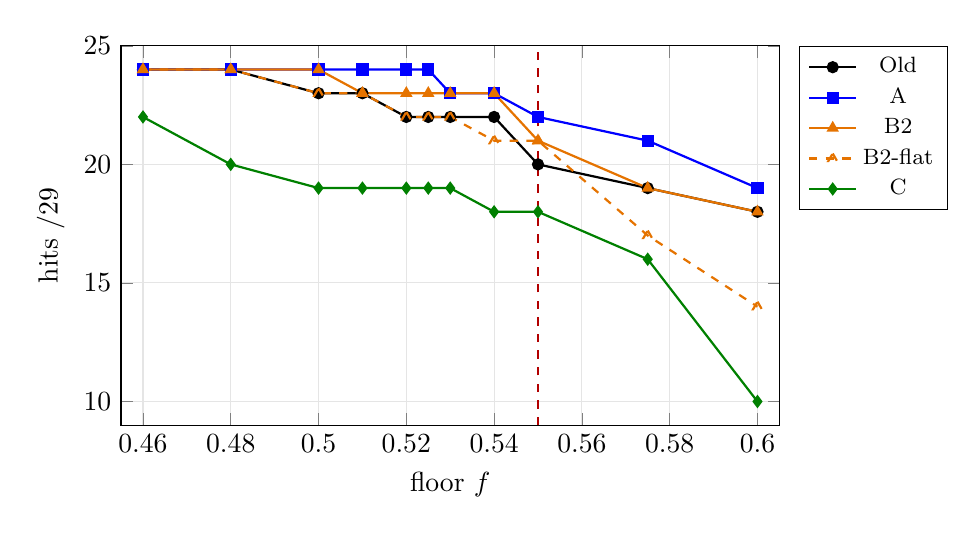
\begin{tikzpicture}
\begin{axis}[width=0.82\linewidth, height=6.4cm, xlabel={floor $f$}, ylabel={hits /29}, ymin=9, ymax=25,
  xmin=0.455, xmax=0.605, xtick={0.46,0.48,0.50,0.52,0.54,0.56,0.58,0.60},
  xticklabel style={/pgf/number format/fixed, /pgf/number format/precision=2},
  legend pos=outer north east, legend style={font=\footnotesize}, grid=major, grid style={gray!20}]
\addplot[black, mark=*, thick, mark size=1.8pt] coordinates {(0.46,24) (0.48,24) (0.5,23) (0.51,23) (0.52,22) (0.525,22) (0.53,22) (0.54,22) (0.55,20) (0.575,19) (0.6,18)};
\addlegendentry{Old}
\addplot[blue, mark=square*, thick, mark size=1.8pt] coordinates {(0.46,24) (0.48,24) (0.5,24) (0.51,24) (0.52,24) (0.525,24) (0.53,23) (0.54,23) (0.55,22) (0.575,21) (0.6,19)};
\addlegendentry{A}
\addplot[orange!90!black, mark=triangle*, thick, mark size=1.8pt] coordinates {(0.46,24) (0.48,24) (0.5,24) (0.51,23) (0.52,23) (0.525,23) (0.53,23) (0.54,23) (0.55,21) (0.575,19) (0.6,18)};
\addlegendentry{B2}
\addplot[orange!90!black, dashed, mark=triangle, thick, mark size=1.8pt] coordinates {(0.46,24) (0.48,24) (0.5,23) (0.51,23) (0.52,22) (0.525,22) (0.53,22) (0.54,21) (0.55,21) (0.575,17) (0.6,14)};
\addlegendentry{B2-flat}
\addplot[green!50!black, mark=diamond*, thick, mark size=1.8pt] coordinates {(0.46,22) (0.48,20) (0.5,19) (0.51,19) (0.52,19) (0.525,19) (0.53,19) (0.54,18) (0.55,18) (0.575,16) (0.6,10)};
\addlegendentry{C}

  \addplot[red!70!black, thin, dashed] coordinates {(0.55,9) (0.55,25)};
\end{axis}
\end{tikzpicture}
\caption{Hits against the floor. Every design gains as the floor drops; A's curve is simply shifted right (its peaks are
higher). The default floor (dashed) happens to sit where A is ahead.}
\label{fig:sweep}
\end{figure}

\begin{table}[ht]
\centering\small
\begin{tabular}{@{}lccc@{}}
\toprule
Design & best hits with $\le$1 FP & best hits with $\le$2 FP & at default floor \\
\midrule
Old     & 19 (0.575) & 23 (0.51) & 20 / 2 FP \\
A       & 19 (0.60)  & 22 (0.55) & 22 / 2 FP \\
B2      & 18 (0.60)  & 23 (0.51--0.54) & 21 / 2 FP \\
B2 flat & \textbf{21} (0.54--0.55) & \textbf{24} (0.46--0.48) & 21 / 1 FP \\
C (C2)  & 20 (0.48)  & 20 (0.48) & 19 / 1 FP (C2) \\
\bottomrule
\end{tabular}
\caption{Each design at its best floor for a given number of false detections (6 absent objects). Read off
Table~\ref{tab:sweep}.}
\label{tab:opPoint}
\end{table}

\paragraph{What the sweep shows.}
\begin{itemize}
  \item \textbf{The floor matters more than the teacher.} Between 0.46 and 0.60 every design moves by 5--12 hits; at a
        matched operating point the designs differ by at most 2--3.
  \item \textbf{B2 flat has the best trade-off} (24/29 with 2 FP; 21/29 with 1 FP) and is the only design that ever
        finds the keyboard. Its segment-shaped features separate present from absent objects better at low floors.
  \item \textbf{The level choice costs false positives}: B2 reaches 24 hits only with 4--5 false detections, B2 flat with 2.
        For A, both versions need 5 false detections to reach 24.
  \item \textbf{ViT-L/14 is the most conservative}: few false positives (none on flightroom at 0.48), but it never exceeds
        22 hits; its absent-object peaks are lowest (mean 0.472) but so are its present-object peaks (0.587).
  \item \textbf{Two ``absent'' objects fire for every design at every floor}: \emph{ceiling fan} (backroom) and
        \emph{recycling bin} (flightroom). Look-alikes are probably present (a ceiling fixture; a bin-like container).
        The negative set needs the same ground-truth check the positives had.
  \item \textbf{Caveat.} With 29 present and 6 absent objects, one query is 3.4 points of hit rate; A's +3/$-$1 against Old
        has a two-sided sign-test $p\approx0.63$. None of the differences between designs is statistically significant.
\end{itemize}

\subsection{B $\rightarrow$ B2: what the fallback and levels did}
\begin{itemize}
  \item \textbf{The fallback fixed FMGS's collapse.} B left 0-vectors in uncovered cells; FMGS learned them, its CLIP
        output shrank towards zero over large areas, and relevancy there became flat (B F-C on flightroom: 1/16). With the
        pyramid in those cells, B2's F-C recovers to 6/16 on flightroom (12/29 overall).
  \item \textbf{It also fixed thin structures on the lift}: office chair, round table and PVC pipe frame come back,
        because the cells around thin objects --- poorly covered by SAM --- now carry the pyramid's evidence.
  \item \textbf{The levels add nothing} (B2 21 = B2 flat 21 at 0.55; worse trade-off in the sweep). Most cells of the
        \emph{part} and \emph{region} maps are fallback cells, so the three maps are largely the same pyramid with small
        differences; choosing the maximum mainly adds the max-of-three bias of Section~\ref{sec:floor}.
\end{itemize}

\subsection{C $\rightarrow$ C2: calibration helps a little, the larger CLIP does not}
\begin{itemize}
  \item The calibrated floor (0.5222) gains armchair, red cup and water bottle across backends and loses nothing (lift
        18 $\rightarrow$ 19, F-C 8 $\rightarrow$ 10). The per-scene floors differ (0.498 vs 0.546), so a single model-wide floor
        is still a compromise.
  \item ViT-L/14 does not fix the recognition misses: keyboard (peak 0.49) and floor lamp (0.49) stay below even the
        calibrated floor, and it newly misses office chair and purple foam mat. Its crops are still $224\times224$ squares,
        so the coarseness problem is unchanged, and it costs 6--7$\times$ the teacher time.
  \item Its FMGS ran with PyTorch heads (tiny-cuda-nn out of memory at 768-d), so its FMGS numbers also reflect a
        slower, differently-initialised head.
\end{itemize}

\subsection{Why FMGS trails the lift}
\label{sec:fmgs}
FMGS's misses are mostly ``no candidate'' (F-CD: 15--21 of 29), but unlike the lift's they are \emph{not} caused by low
peaks: the mean peak of F-CD's no-candidate queries is 0.57--0.61, above the floor. Inspecting three such queries on
flightroom (Old F-CD) shows why:

\begin{table}[ht]
\centering\small
\begin{tabular}{@{}llcccc@{}}
\toprule
Query & Table & Peak & \shortstack{Gaussians\\$\ge\tau$} & \shortstack{Spread of\\top-100 (m)} & \shortstack{Top-100 inside camera\\volume $\pm$1\,m} \\
\midrule
garden cart   & FMGS & 0.614 & 75  & 6.50 & 69\,\% \\
              & lift & 0.621 & 113 & 0.24 & 100\,\% \\
cardboard box & FMGS & 0.638 & 101 & 7.51 & 62\,\% \\
              & lift & 0.619 & 194 & 0.69 & 90\,\% \\
water bottle  & FMGS & 0.613 & 103 & 5.75 & 69\,\% \\
              & lift & 0.604 & 143 & 0.05 & 100\,\% \\
\bottomrule
\end{tabular}
\caption{FMGS's highest-relevancy Gaussians are scattered across the room (and a third lie outside the region the
cameras cover), so no 0.1\,m voxel cluster reaches the 15-Gaussian minimum. The lift's are compact.}
\end{table}

Contributing causes:
\begin{itemize}
  \item \textbf{Speckle from the hash field} (likely cause, not yet isolated). The field is queried at \emph{all} 380--530\,k centres but trained only on the
        most opaque 40\,\%; the fine levels and hash collisions give isolated high values at untrained points, especially
        outside the camera volume where there was no supervision at all. The relative threshold is then set by these
        outliers.
  \item \textbf{DINO dominates the loss.} With weights 0.2/0.8, the CLIP term flattens at $\sim10^{-4}$ within 250 steps
        while DINO keeps falling; F-C (CLIP only) is consistently better than F-CD (15 vs 11 for Old).
  \item \textbf{Per-group heads split capacity} (A, B2): F-CD drops from 11 to 8 (A) and 6 (B2); each head sees a third of
        the steps.
  \item \textbf{Smoothing}: the field interpolates over space, so small objects (red cup, water bottle) blur into their
        surroundings; the lift keeps per-Gaussian detail.
\end{itemize}

\subsection{L-CD (DINO at query time)}
L-CD is neutral on average (Old 20 = 20, A 22 = 22, B2 21 = 21, C2 19 $\rightarrow$ 18). Diffusion over DINO-weighted
neighbours helps where relevancy is patchy within one object (A's L-CD finds the swivel chair, the only design to do so)
and hurts where an object borders a similar-looking neighbour: A's L-CD loses the water jug (bad position), B2's the
upholstered chair and C2's the armchair. With B it hurt badly (19 $\rightarrow$ 15); a likely cause is that B's sparser,
segment-shaped features give DINO-weighted neighbourhoods with little CLIP evidence, which diffusion averages in.

\subsection{The queries nobody finds}
\begin{itemize}
  \item \textbf{camera tripod} (peak $\le$0.54 everywhere): a thin, mostly see-through object --- few Gaussians and every
        crop around it is mostly background. Found by no design at any floor.
  \item \textbf{keyboard} (0.49--0.52) and \textbf{floor lamp} (0.49--0.56): CLIP recognition limits measured on centred
        crops too; only B2 flat at floors $\le$0.48 finds the keyboard.
  \item \textbf{white bucket} (wrong object, 1.8--3.7\,m away): the top candidate is a white ceiling fixture --- colour and
        shape dominate CLIP's notion of ``white bucket''; no height or size prior is used.
  \item \textbf{drone gate} (wrong object, $\approx$5\,m away): the candidate is a tripod by the far window. ``Drone gate'' is
        a domain term CLIP has rarely seen; it matches generic frames and stands.
\end{itemize}

%=======================================================================================
\section{Proposals}
%=======================================================================================

\subsection{For every design: the query}
\begin{enumerate}
  \item \textbf{Calibrate the floor per table and scoring rule, without evaluation queries.} C2's quantile mapping over a
        neutral vocabulary is the template; it must be applied to the score the query actually uses (for A/B2: the
        best-group relevancy, not the averaged rows). Better still: calibrate to a target false-positive rate on a
        larger, verified set of absent objects.
  \item \textbf{Fix the max-of-three bias} in A/B2: either calibrate each group's relevancy (per-group quantile
        normalisation before taking the maximum) or replace the hard maximum by a softmax-weighted average of groups.
  \item \textbf{Verify the negative set} (ceiling fan, recycling bin) as the positives were; grow it to 15+ absent
        objects per scene so false-positive rates are measurable.
  \item \textbf{Prompt ensembling} (``a photo of a \{\}'', ``a \{\} in a room'', synonyms) for the text side: cheap and
        model-agnostic (the CLIP paper reports a few points of ImageNet accuracy from it); most relevant to domain terms (drone gate).
  \item \textbf{Geometric priors} from the instruction (Phase~6 parser): expected size and height (``bucket'' $\Rightarrow$
        floor-level, $<$0.5\,m) to re-rank candidates; would fix white bucket's ceiling fixture.
\end{enumerate}

\subsection{Old (pyramid)}
\begin{itemize}
  \item Cheapest design (3--4\,min lift, 0.9\,GB table, 0.5--0.8\,s query) and, with a properly calibrated floor, as good as
        A. If A's extra cost is not justified by a calibrated comparison, Old with a calibrated floor is the efficient
        default.
  \item Weight scales by crop--object fit instead of equally (e.g.\ weight each crop by its CLIP confidence against the
        canonical negatives), keeping one map.
\end{itemize}

\subsection{A (multi-scale)}
\begin{itemize}
  \item Calibrate per group (above). Then the per-query choice can show whether it helps beyond the bias.
  \item Reduce cost: store the groups in fp8 or PCA-compressed (512 $\rightarrow$ 128), or lift only the groups and drop
        \code{clip}; compute the three relevancies in one pass (query 2.0--2.7\,s $\rightarrow$ $<$1\,s).
\end{itemize}

\subsection{B2 (SAM regions)}
\begin{itemize}
  \item \textbf{Adopt B2 flat as the B-design}: best operating point in the sweep, same table, 4$\times$ faster query.
  \item \textbf{Coverage-weighted lift}: carry the SAM coverage fraction into the lift weight, so pixels with a real segment
        embedding count more than fallback pixels.
  \item \textbf{Better masks for thin objects}: more prompt points (64$\times$64) or SAM~2 / a hierarchical segmenter;
        multi-view-consistent masks (Gaussian Grouping style) so one object gets one embedding across views.
  \item \textbf{Storage}: 37\,GB of teacher maps for two scenes is unsustainable; store segment embeddings + mask indices
        (a few MB per photo) and paint the grid on the fly in the lift.
  \item For FMGS: also mask fallback cells out of the CLIP loss (or down-weight them) instead of training on pyramid
        targets.
\end{itemize}

\subsection{C2 (ViT-L/14)}
\begin{itemize}
  \item Do not use ViT-L/14 as a dense teacher: 6--7$\times$ cost for no gain here.
  \item \textbf{Use it as a re-ranker} instead: take the top 3--5 candidates of the lift (ViT-B/16), render each candidate's
        box from the two best training views, crop and score with ViT-L/14 (or ViT-L/14-336). Seconds per query, no
        teacher rebuild, targets wrong-object errors.
  \item Per-scene calibration (0.498 vs 0.546) suggests calibrating per table, not per model.
\end{itemize}

\subsection{FMGS}
\begin{itemize}
  \item \textbf{Bake only where supervised}: restrict queries to Gaussians inside the camera volume and to the trained
        subset (or opacity / lift-weight above a threshold); expected to remove most scattered peaks.
  \item \textbf{Spatial smoothing at query time} (kNN diffusion as in L-CD, but on CLIP relevancy alone) before
        thresholding; or require the peak to be computed on clustered Gaussians.
  \item \textbf{Rebalance the loss}: normalise each term by its running magnitude, or raise the CLIP weight; train the CLIP
        head longer.
  \item \textbf{Initialise or supervise from the lift}: a 3D loss pulling the field towards the lift's per-Gaussian
        features gives every trained Gaussian a direct target (cheap, avoids rendering noise).
  \item \textbf{One head, many scales}: condition one CLIP head on the scale (as LERF's field does) instead of separate
        heads.
\end{itemize}

\subsection{Combinations}

\begin{figure}[ht]
\centering
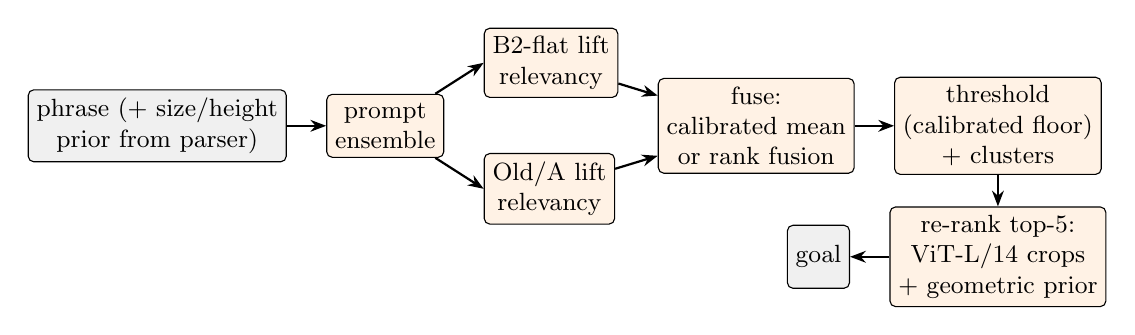
\begin{tikzpicture}[node distance=4mm and 5mm, font=\small]
  \node[data] (q) {phrase (+ size/height\\prior from parser)};
  \node[stp, right=of q] (en) {prompt\\ensemble};
  \node[stp, right=of en, yshift=8mm] (l1) {B2-flat lift\\relevancy};
  \node[stp, right=of en, yshift=-8mm] (l2) {Old/A lift\\relevancy};
  \node[stp, right=of l1, yshift=-8mm] (fu) {fuse:\\calibrated mean\\or rank fusion};
  \node[stp, right=of fu] (cl) {threshold\\(calibrated floor)\\+ clusters};
  \node[stp, below=of cl] (rr) {re-rank top-5:\\ViT-L/14 crops\\+ geometric prior};
  \node[data, left=of rr] (g) {goal};
  \draw[arr] (q) -- (en); \draw[arr] (en) -- (l1.west); \draw[arr] (en) -- (l2.west);
  \draw[arr] (l1) -- (fu); \draw[arr] (l2) -- (fu); \draw[arr] (fu) -- (cl); \draw[arr] (cl) -- (rr); \draw[arr] (rr) -- (g);
\end{tikzpicture}
\caption{A proposed combined pipeline: two complementary lift tables fused at the relevancy level, a calibrated floor,
and a ViT-L/14 re-ranker with geometric priors on a handful of candidates.}
\label{fig:combo}
\end{figure}

\begin{itemize}
  \item \textbf{Ceiling.} The union of all designs' lift hits at the default floor is 24/29, the same as B2 flat alone at
        its best floor; a combination of teachers can gain at most one or two objects on these sets. Teacher
        combinations alone are not worth 10+ GPU hours.
  \item \textbf{B2 flat + Old/A (relevancy fusion)}: both tables already exist; fusing calibrated relevancies (mean, or
        rank-based) is a query-time change. The designs fail on different queries (hose reel vs.\ upholstered chair), so
        fusion should keep the union of their strengths while averaging away their individual false positives.
  \item \textbf{Any lift + ViT-L/14 re-ranker}: the cheapest way to use the larger model where it is strong (rejecting
        absent objects; flightroom AUROC 0.96).
  \item \textbf{A + C (ViT-L/14 multi-scale teachers)}: not recommended --- $\approx$10\,h of teachers for a design whose
        components each showed no calibrated gain.
  \item \textbf{FMGS with B2-flat teachers}, coverage-masked loss, CLIP-weighted loss and supervised-only baking: the
        configuration most likely to close the gap to the lift, if a trained field is still wanted (e.g.\ for querying
        arbitrary 3D points).
\end{itemize}

\begin{table}[ht]
\centering\small
\begin{tabularx}{\linewidth}{@{}lL>{\raggedright\arraybackslash}p{3.3cm}>{\raggedright\arraybackslash}p{3.5cm}@{}}
\toprule
Priority & Proposal & Cost & Expected effect \\
\midrule
1 & Per-table, per-rule floor calibration (neutral vocabulary); verify and enlarge absent-object set & CPU, hours & fair default; +1--3 hits \\
2 & B2 flat as a lift option; relevancy fusion with Old/A & CPU, query-time & best measured trade-off \\
3 & ViT-L/14 crop re-ranker on top-5 candidates & CPU/GPU, seconds per query & fewer wrong objects \\
4 & FMGS: supervised-only baking + query-time smoothing & CPU & most F-* ``no candidate'' misses \\
5 & Prompt ensembles; size/height priors from the Phase~6 parser & CPU & domain terms, white bucket \\
6 & B2 storage (segment ids instead of painted maps), better masks for thin objects & GPU, 1--2\,h & cost; tripod, PVC \\
7 & More scenes and 50+ queries per scene & annotation time & significance \\
\bottomrule
\end{tabularx}
\caption{Proposals in suggested order.}
\end{table}

%=======================================================================================
\section{Conclusions}
%=======================================================================================
\begin{enumerate}
  \item The training-free \textbf{lift beats FMGS} on a frozen splat for every teacher design (19--22 vs 5--15 of 29),
        and FMGS's main failure is spatially scattered high relevancy rather than weak features.
  \item At the default settings \textbf{A} is best (22/29), \textbf{B2} close (21), \textbf{Old} 20, \textbf{C2} 19. But a
        floor sweep shows that the default floor favours A because A's max-over-groups raises all peaks; at an equal
        number of false detections the designs are within 2--3 objects, \textbf{B2 flat} having the best trade-off (24/29 at
        2 of 6 false detections).
  \item B2's pyramid fallback was the right fix for B; its size levels are not needed. Calibrating ViT-L/14's floor (C2)
        helped slightly; the larger model does not address recognition misses and is better used as a re-ranker.
  \item The next gains are in the \emph{query} --- calibration, fusion, re-ranking, priors --- and in a larger, verified
        evaluation set, not in more expensive teachers.
\end{enumerate}

\appendix
\section{Reproducibility}
\begin{table}[ht]
\centering\footnotesize
\begin{tabularx}{\linewidth}{@{}lL@{}}
\toprule
Item & Where \\
\midrule
Old / A & \code{main}; A merged in \code{3345c56} (\code{61d8b5b}); \code{--clip-mode scales} (default for \code{--backend lift}) \\
B / B2 & branch \code{sem/variant-b-sam}: \code{c7c2499} (B), \code{83e0cc0} (B2, \code{--clip-mode sam2}) \\
C / C2 & \code{--clip-model ViT-L-14 --clip-pretrained laion2b\_s32b\_b82k}; C2 on \code{sem/variant-c-clipl} \code{7ac2cb0}
  (\code{scripts/calibrate\_floor.py}) \\
Tables (host) & \code{gsplats/workspace/<scene>/semantics/<run>/}\{\code{lift\_pyr}, \code{lift\_ms}, \code{lift\_sam2},
  \code{lift\_clipl}, \code{fmgs*}\}; official \code{lift} = A \\
Results & \code{docs/phase5\_results/teacher\_variants\_final\_2026-10-08/} (\code{variants.csv}, \code{per\_query.csv},
  \code{floor\_sweep.json}); \code{docs/SEMANTICS.md} \S13--16 \\
Evaluation & \code{python -m radiance\_semantics.evaluate --scene <s> --variants L-C@sam2 L-Cflat@sam2 \dots} \\
Floor sweep & \code{semantics/scripts/floor\_sweep.py --tables Old=lift\_pyr A=lift\_ms A-flat=lift\_ms:flat \dots} \\
Query sets & \code{docs/phase5\_queries/} (frozen \code{f38225b}; amended backroom 7~Oct) \\
Host & intellisense08, RTX~2080 8\,GB, driver 535, kitchen env (torch 2.1.2 / CUDA 11.8) \\
\bottomrule
\end{tabularx}
\end{table}

\FloatBarrier
\begin{thebibliography}{9}
\bibitem{lerf} J.~Kerr, C.~M.~Kim, K.~Goldberg, A.~Kanazawa, M.~Tancik. \emph{LERF: Language Embedded Radiance Fields.} ICCV 2023.
\bibitem{fmgs} X.~Zuo, P.~Samangouei, Y.~Zhou, Y.~Di, M.~Li. \emph{FMGS: Foundation Model Embedded 3D Gaussian Splatting for Holistic 3D Scene Understanding.} IJCV 2024.
\bibitem{langsplat} M.~Qin, W.~Li, J.~Zhou, H.~Wang, H.~Pfister. \emph{LangSplat: 3D Language Gaussian Splatting.} CVPR 2024.
\bibitem{occam} J.~Cheng, J.-N.~Zaech, L.~Van~Gool, D.~P.~Paudel. \emph{Occam's LGS: An Efficient Approach for Language Gaussian Splatting.} 2024.
\bibitem{ludvig} J.~Marrie, R.~M\'en\'egaux, M.~Arbel, D.~Larlus, J.~Mairal. \emph{LUDVIG: Learning-free Uplifting of 2D Visual Features to Gaussian Splatting Scenes.} 2024.
\bibitem{sam} A.~Kirillov et al. \emph{Segment Anything.} ICCV 2023.
\bibitem{clip} A.~Radford et al. \emph{Learning Transferable Visual Models From Natural Language Supervision.} ICML 2021.
\bibitem{dinov2} M.~Oquab et al. \emph{DINOv2: Learning Robust Visual Features without Supervision.} TMLR 2024.
\end{thebibliography}

\end{document}
